\documentclass[11pt,a4paper]{article}

\usepackage[utf8]{inputenc}
\usepackage[T1]{fontenc}
\usepackage{lmodern}
\usepackage[margin=2.5cm]{geometry}
\usepackage{amsmath,amssymb}
\usepackage{graphicx}
\usepackage{booktabs}
\usepackage{caption}
\usepackage[authoryear,round]{natbib}
\usepackage[hidelinks]{hyperref}

\graphicspath{{figures/}}
\newcommand{\dEVE}{$\Delta$EVE}
\newcommand{\dNII}{$\Delta$NII}

\title{Interest Rate Risk in the Banking Book of a Swiss Cantonal Bank\\
\large Rebuilding the FINMA Shock Test of Banque Cantonale Vaudoise from Public Data}
\author{Andreas Kyrlakis\\
\small MSc in Finance, HEC Lausanne (University of Lausanne)}
\date{November 2026}

\begin{document}
\maketitle

\begin{abstract}
\noindent
Swiss banks fund long fixed-rate mortgages with deposits that clients can withdraw at any time. FINMA measures the resulting interest rate risk with six standard shocks and flags a bank as an outlier when the fall in the economic value of equity (\dEVE) exceeds 15\% of Tier~1 capital. This paper rebuilds the banking book of Banque Cantonale Vaudoise (BCV) at 31 December 2025 from the 18 lines of its public repricing table (IRRBBA1), prices it on a CHF curve fitted to Confederation bonds and SARON (fit error 1.8 basis points), and compares the result with the figures BCV published (IRRBB1). The model reproduces the two parallel shocks within 4\% and 7\% ($-449$ versus $-467$ and $+454$ versus $+488$ CHF million) and gives a worst \dEVE{} of 12.9\% of Tier~1 against 13.4\% published. Under the shock sizes of FINMA's 2028 consultation draft the ratio reaches 15.0\%. The result rests on the deposit model: halving the stable share of sight deposits raises the loss to 19.3\% of Tier~1, and the six published figures are best matched by fully stable sight deposits and short-lived savings. BCV's existing payer swaps halve the exposure (29.9\% without them), and a further CHF 1.39 billion 5-year swap would bring it to 10\%. Pass-through estimated on SNB data is 0.35 for savings and 0.01 for payment accounts. Because client rates are close to zero, the model loses 158 million of net interest income when rates fall, against 3 million in BCV's figure, which assumes negative rates can be passed on. Finally, the prepayment penalty that Swiss lenders charge is worth a lot: without it, a moderate refinancing response would turn the 454 million gain of the down shock into a loss.
\end{abstract}

\section{Introduction}

A bank that lends at a fixed rate for several years and borrows at rates that reset quickly is exposed to rising rates. In its \emph{economic value} view, the present value of the assets falls more than that of the liabilities; in its \emph{earnings} view, funding costs rise before asset yields do. The Basel Committee's standard on interest rate risk in the banking book \citep[IRRBB,][]{bcbs2016} asks banks to measure both effects under six prescribed shocks, and FINMA applies it in Circular 2019/2 \citep{finma2019}. Since 2019, Swiss banks publish the results in two Pillar~3 tables: IRRBBA1, which describes the repricing structure of the balance sheet, and IRRBB1, which gives \dEVE{} and \dNII{} for each shock.

This project asks a simple question: \emph{can an outsider reproduce a bank's published interest rate risk from its public disclosure, and which assumptions drive the answer?} It uses Banque Cantonale Vaudoise (BCV), a large cantonal bank listed on SIX, with CHF 60.6 billion of total assets in its parent-company accounts. BCV is a good case: mortgages are 57\% of its balance sheet, sight and savings deposits 50\%, and its published \dEVE{} has stayed close to the 15\% outlier threshold since 2024.

The paper proceeds in five steps: (i) turn the repricing table into cash flows; (ii) build a CHF curve and the six FINMA shocks; (iii) compute \dEVE{} and \dNII{} and compare them with the published numbers; (iv) explain the gaps and test the sensitivity to the deposit model; (v) study two management questions, the mortgage prepayment option and a hedging swap.

\section{Regulatory framework}

\paragraph{Economic value.} For a set of cash flows $CF_i$ at times $t_i$, discounted on a zero curve $r(t)$, the economic value is $EV = \sum_i CF_i\, e^{-r(t_i) t_i}$. Equity is excluded, so EV is the value of the banking book that belongs to shareholders. For a shock $\Delta_s(t)$,
\begin{equation}
\Delta EVE_s = \sum_i CF_i \left( e^{-(r(t_i)+\Delta_s(t_i))\,t_i} - e^{-r(t_i)\,t_i} \right).
\end{equation}

\paragraph{The six shocks.} Following \citet{bcbs2016} (SRP31.90--93), with $x = 4$ years:
\begin{align*}
\text{parallel: } & \pm \bar R, \qquad \text{short: } \pm \bar S\, e^{-t/x}, \qquad \text{long: } \bar L\,(1-e^{-t/x}),\\
\text{steepener: } & -0.65\,|\text{short}| + 0.9\,|\text{long}|, \qquad \text{flattener: } +0.8\,|\text{short}| - 0.6\,|\text{long}|.
\end{align*}
For CHF, FINMA sets $\bar R = 150$, $\bar S = 150$ and $\bar L = 100$ basis points and applies no floor to post-shock rates \citep{finma2019}. The consultation draft of 4 November 2026 raises the CHF parallel shock to 175 and the short shock to 250 basis points from 2028. Our implementation reproduces FINMA's printed table exactly (for example $-97$, $+120$ and $+137$ bp for the steepener, flattener and short-up shocks in buckets 1, 1 and 4; Table~\ref{tab:shocks}).

\paragraph{Net interest income.} \dNII{} is the change in net interest income over 12 months on a constant balance sheet after an instantaneous parallel shock.

\paragraph{Outlier test.} A bank is an outlier when the largest fall in EVE over the six shocks reaches 15\% of Tier~1 capital. FINMA then assesses the bank case by case.

\begin{table}[h]
\centering
\caption{CHF shocks at selected FINMA bucket midpoints (bp), as computed by \texttt{src/shocks.py}.}
\label{tab:shocks}
\begin{tabular}{lrrrrrrrrr}
\toprule
Bucket & O/N & 1M & 6M & 1Y & 2Y & 3Y & 5Y & 10Y & $>$20Y \\
\midrule
Parallel up & 150 & 150 & 150 & 150 & 150 & 150 & 150 & 150 & 150 \\
Steepener & $-97$ & $-96$ & $-81$ & $-61$ & $-31$ & $-10$ & 29 & 73 & 90 \\
Flattener & 120 & 118 & 104 & 85 & 56 & 36 & $-2$ & $-43$ & $-60$ \\
Short up & 150 & 148 & 137 & 121 & 97 & 80 & 49 & 14 & 0 \\
\bottomrule
\end{tabular}
\end{table}

\section{Data}

All inputs are public and need no account; the code downloads them again.
\begin{itemize}
  \item \textbf{BCV Pillar 3 at 31.12.2025} \citep{bcvpillar3}: Table 26 (IRRBBA1, p.~53--54) gives, for 18 balance-sheet lines of the parent bank, the volume and the average repricing date, and for non-maturity positions the maximum repricing date; Table 27 (IRRBB1, p.~57) gives \dEVE{} and \dNII{} at 31.12.2025 and 30.06.2025 and Tier~1 capital (CHF 3,484 million). The report also describes BCV's methods (p.~55--56): SARON-swap discounting, replication of deposits on 1-month to 10-year rates with a volatile part placed at one month, a compensation penalty on early repayments, and no automatic options. The 2024 report \citep{bcvpillar3b} gives the two previous dates.
  \item \textbf{BCV annual report 2025} \citep{bcvar}: parent balance sheet and income statement (p.~176--177), used for consistency checks.
  \item \textbf{SNB data portal} \citep{snbdata}: SARON fixing; yields and residual maturities of the 22 Confederation bonds quoted on 30 December 2025 (last day of 2025 with quotes); eight-year yields of cantonal and Pfandbrief bonds; and client rates on new business (mortgages by term, payment accounts, savings).
\end{itemize}
The transcribed IRRBBA1 lines add up to CHF 3,516 million against a published net total of 3,517 (rounding). Table~\ref{tab:check} compares them with the balance sheet: the gaps are below 1.2\%. One published figure is inconsistent: the CHF part of savings deposits ($-15{,}889$) exceeds the total ($-13{,}319$); we use the total.

\begin{table}[h]
\centering
\caption{The repricing table against the audited balance sheet (CHF million).}
\label{tab:check}
\begin{tabular}{lrrr}
\toprule
 & IRRBBA1 & Annual report & Gap \\
\midrule
Mortgages (fixed, money-market, variable) & 34,771 & 34,829 & $-0.2\%$ \\
Customer deposits (term, sight, savings) & 37,087 & 37,212 & $-0.3\%$ \\
Pfandbrief loans & 11,238 & 11,143 & $+0.9\%$ \\
Financial investments & 7,337 & 7,423 & $-1.2\%$ \\
Other claims vs liquidity & 8,472 & 8,478 & $-0.1\%$ \\
\bottomrule
\end{tabular}
\end{table}

\section{Method}

\subsection{From the repricing table to cash flows}

Each line with a contractual repricing date becomes a \emph{ladder}: monthly tranches with maturities spread uniformly over $(0, 2\bar m]$, where $\bar m$ is the published average, so the average matches by construction. Each tranche is a bullet loan with monthly coupons. Fixed-rate mortgages (CHF 34.2 billion, $\bar m = 4.0$ years) therefore run up to 8 years, financial investments up to 12 years and Pfandbrief loans up to 13.6 years. The swap lines show BCV's hedges: receive legs of CHF 12.9 billion reprice in 0.3 years on average (floating) and pay legs in 3.5 years (fixed): BCV pays fixed. Money-market mortgages, SNB sight deposits (``other claims'') and other liabilities reprice overnight.

\paragraph{Coupons.} The coupon of a line is the average SNB rate for comparable new business over its origination window: 8-year fixed mortgages over 8 years (1.81\%), 7-year over 6.6 years for fixed customer loans (1.83\%), cantonal bonds over 12 years for financial investments (0.35\%), Pfandbrief bonds over 13.6 years (0.52\%), and the 7-year Confederation yield over 7 years as a proxy for the fixed rate of BCV's swaps (0.10\%). Short positions carry the 30 December 2025 rate.

\subsection{Non-maturity deposits}

Sight deposits (CHF 17.1 billion) and savings (CHF 13.3 billion) have no maturity. As is standard \citep{jarrow1998,kalkbrener2004}, their rate sensitivity is modelled by a \emph{replicating portfolio}: a volatile part that reprices at once and a stable part spread over a ladder of tenors. BCV publishes an average of 1.8 years for both and a maximum of 5 years (sight) and 10 years (savings). With a uniform ladder up to the maximum $M$, the stable share $s$ satisfies $s M/2 = 1.8$, so $s = 72\%$ for sight and $36\%$ for savings.

For earnings, the question is how fast client rates follow market rates \citep{hutchison1996,drechsler2017}. We regress the SNB monthly average rate on new business on SARON over June 2022 -- December 2025 (43 months, a full hiking and cutting cycle):
\begin{center}
\begin{tabular}{lrrrr}
\toprule
SNB series & $\beta$ & $R^2$ & $\beta$ up-cycle & $\beta$ down-cycle \\
\midrule
Savings deposits & 0.35 & 0.75 & 0.39 & 0.38 \\
Private payment accounts & 0.01 & 0.72 & 0.01 & 0.02 \\
Variable mortgages & 0.11 & 0.40 & 0.19 & 0.12 \\
\bottomrule
\end{tabular}
\end{center}
The cycle betas divide the change in client rate by the change in SARON between June 2022, December 2023 and December 2025. Savings rates follow about a third of SARON moves, payment accounts almost none (Figure~\ref{fig:passthrough}). This low beta is what makes deposits a long-duration liability in practice \citep{drechsler2021}.

\subsection{Curve}

The CHF curve is a \citet{svensson1994} extension of \citet{nelson1987} fitted by weighted least squares to the SARON fixing ($-0.04\%$) and the 22 Confederation bond yields of 30 December 2025 (1.5 to 38.5 years); yields to maturity are used as approximate zero rates. The fit error is 1.8 basis points (maximum 4.1). The curve rises from $-0.04\%$ overnight to 0.10\% at 5 years and 0.32\% at 10 years (Figure~\ref{fig:curve}). BCV discounts with SARON swaps, which are not free; a $+20$ bp parallel spread changes \dEVE{} by at most 2 million.

\begin{figure}[t]
\centering
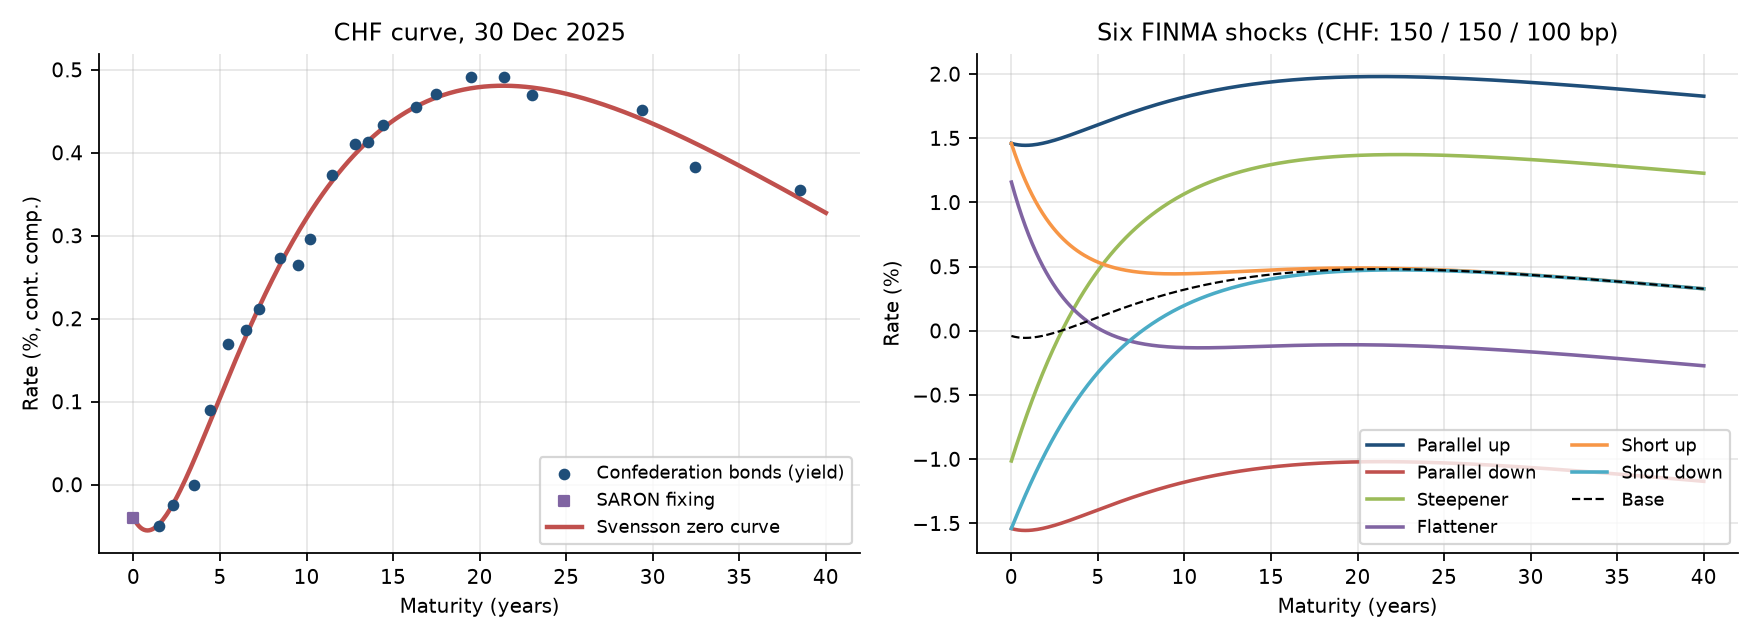
\includegraphics[width=\textwidth]{fig1_curve_and_shocks.png}
\caption{Left: Confederation bond yields, SARON and the fitted zero curve on 30 December 2025. Right: the six FINMA shocks applied to it.}
\label{fig:curve}
\end{figure}

\begin{figure}[t]
\centering
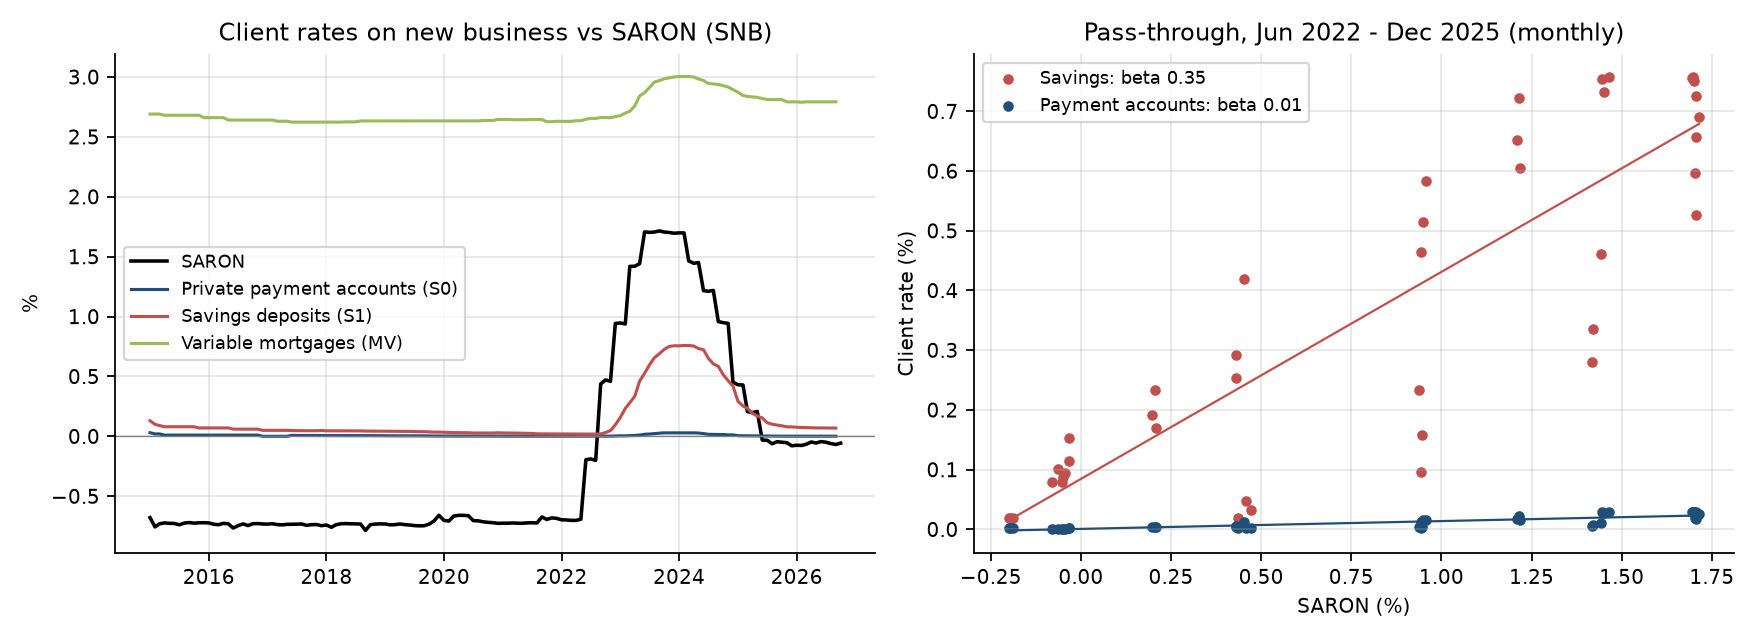
\includegraphics[width=\textwidth]{fig2_deposit_pass_through.png}
\caption{Left: client rates on new business and SARON (SNB). Right: monthly pass-through regressions, June 2022 -- December 2025.}
\label{fig:passthrough}
\end{figure}

\subsection{Earnings}

For \dNII, every tranche that reprices within 12 months is rolled over at a rate moved by the shock for the rest of the year; administered rates (sight, savings, variable mortgages) move at once by $\beta$ times the shock, and deposit rates cannot fall below zero. This floor is the main modelling choice for the down shock, and we report results with and without it.

\section{Results}

\subsection{Repricing gap}

Figure~\ref{fig:gap} shows the resulting repricing profile. The overnight bucket is short CHF 5.6 billion (volatile deposits exceed SNB sight deposits and money-market mortgages), while the 6- to 8-year buckets are long because fixed mortgages and loans are not fully matched by the swaps (which stop at 7 years) or the deposit replication. Beyond 9 years the book is short again through Pfandbrief funding and savings replication.

\begin{figure}[t]
\centering
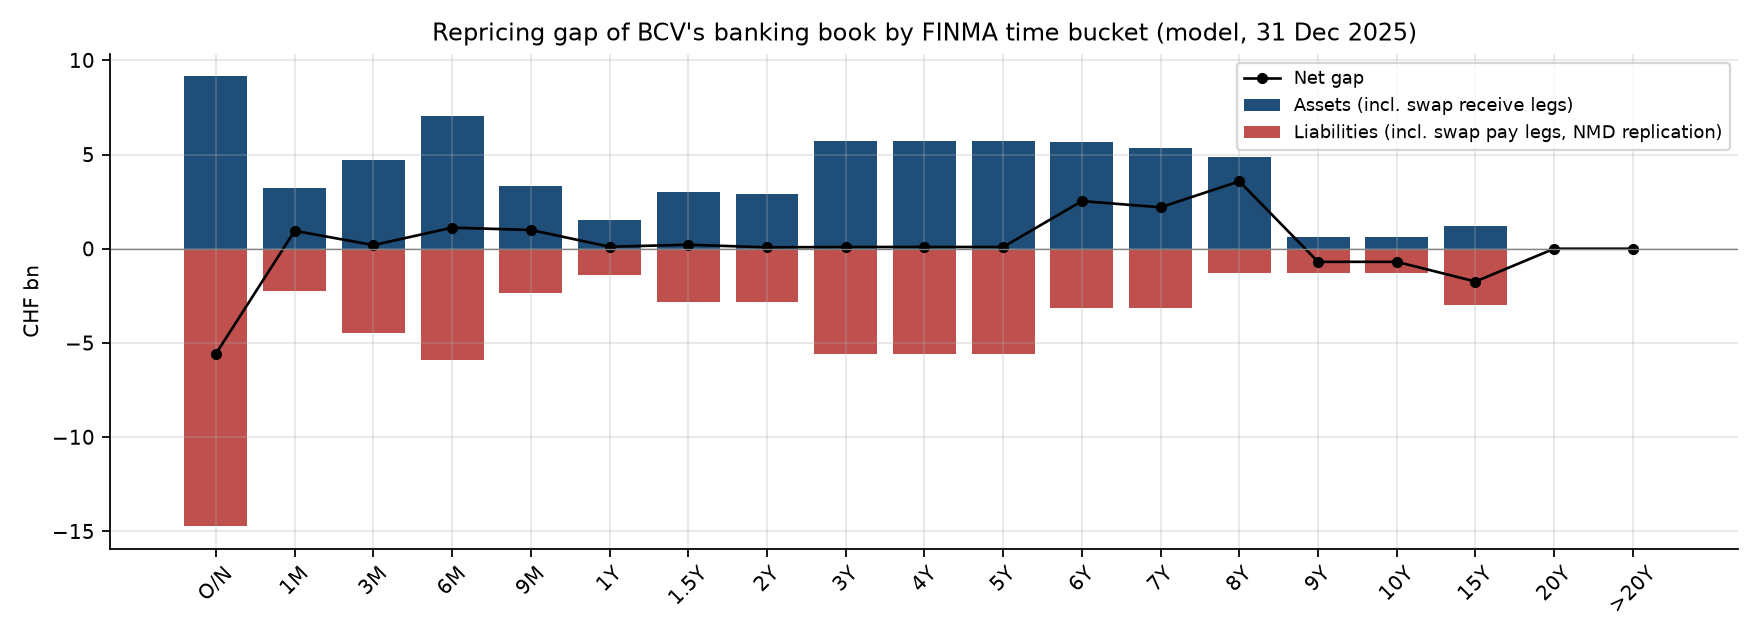
\includegraphics[width=\textwidth]{fig3_repricing_gap.png}
\caption{Repricing gap of the modelled banking book by FINMA time bucket.}
\label{fig:gap}
\end{figure}

\subsection{Model against published figures}

Table~\ref{tab:results} and Figure~\ref{fig:compare} compare the model with IRRBB1. The two parallel shocks, which dominate the outlier test, are reproduced within 4\% and 7\%. The economic value of the banking book is CHF 6.0 billion in the model; the parallel-up shock removes 449 million, i.e.\ 12.9\% of Tier~1 against 13.4\% published. Figure~\ref{fig:position} shows where the loss comes from: fixed mortgages lose CHF 2.1 billion, financial investments and fixed loans 0.9 billion together, while Pfandbrief funding (1.1 billion), the payer swaps (0.6 billion net of their receive legs) and the deposit replication (0.8 billion) offset about 85\% of it.

\begin{table}[h]
\centering
\caption{\dEVE{} and \dNII{} at 31 December 2025, CHF million (Tier 1: 3,484).}
\label{tab:results}
\begin{tabular}{lrrrrr}
\toprule
 & \multicolumn{3}{c}{\dEVE} & \multicolumn{2}{c}{\dNII} \\
\cmidrule(lr){2-4}\cmidrule(lr){5-6}
Scenario & Model & BCV & \% Tier 1 (model) & Model & BCV \\
\midrule
Parallel up & $-449$ & $-467$ & $-12.9$ & 96 & 78 \\
Parallel down & 454 & 488 & 13.0 & $-158$ & $-3$ \\
Steepener & $-41$ & $-138$ & $-1.2$ & & \\
Flattener & $-49$ & 40 & $-1.4$ & & \\
Short up & $-187$ & $-120$ & $-5.4$ & & \\
Short down & 191 & 125 & 5.5 & & \\
\bottomrule
\end{tabular}
\end{table}

\begin{figure}[t]
\centering
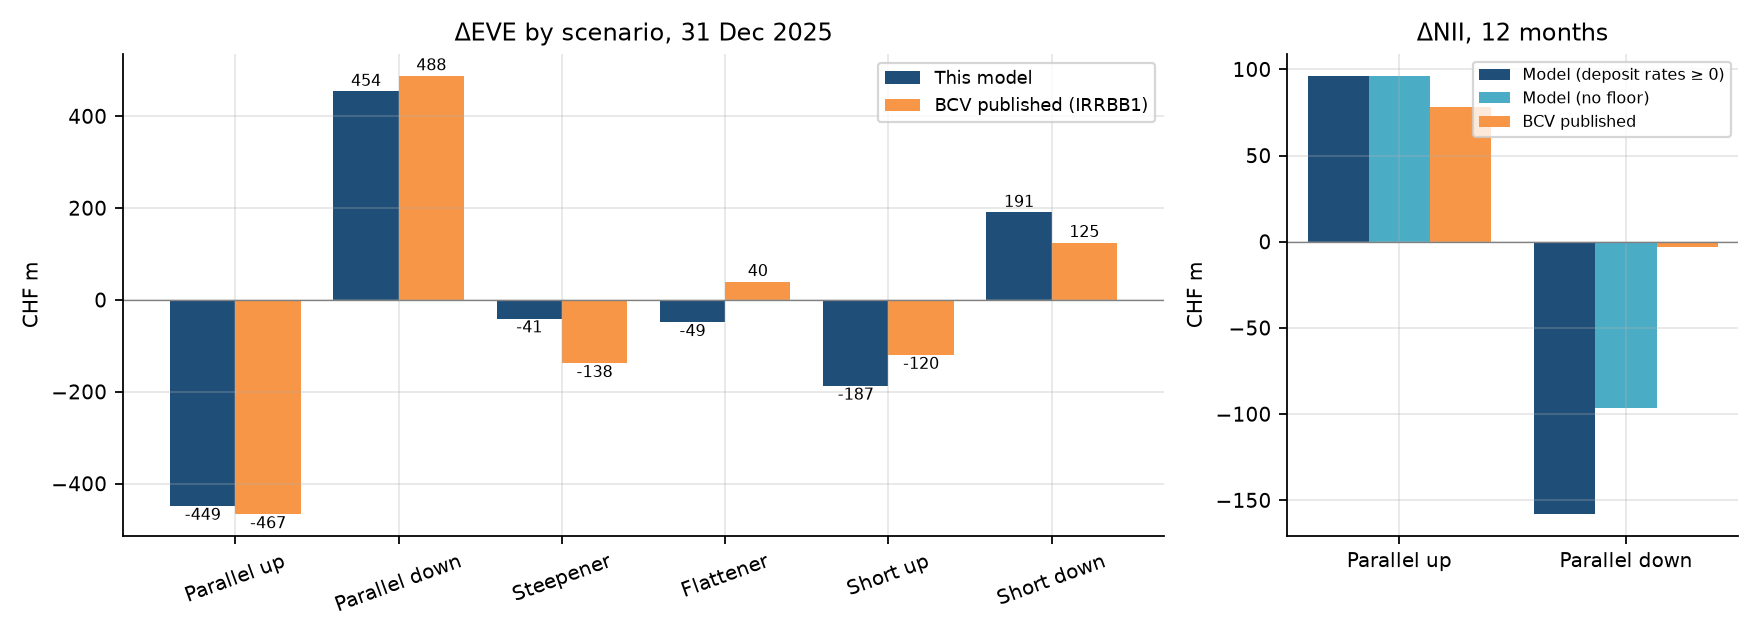
\includegraphics[width=\textwidth]{fig4_model_vs_published.png}
\caption{Model against BCV's published IRRBB1 table. \dNII{} is shown with and without a zero floor on deposit rates.}
\label{fig:compare}
\end{figure}

\begin{figure}[t]
\centering
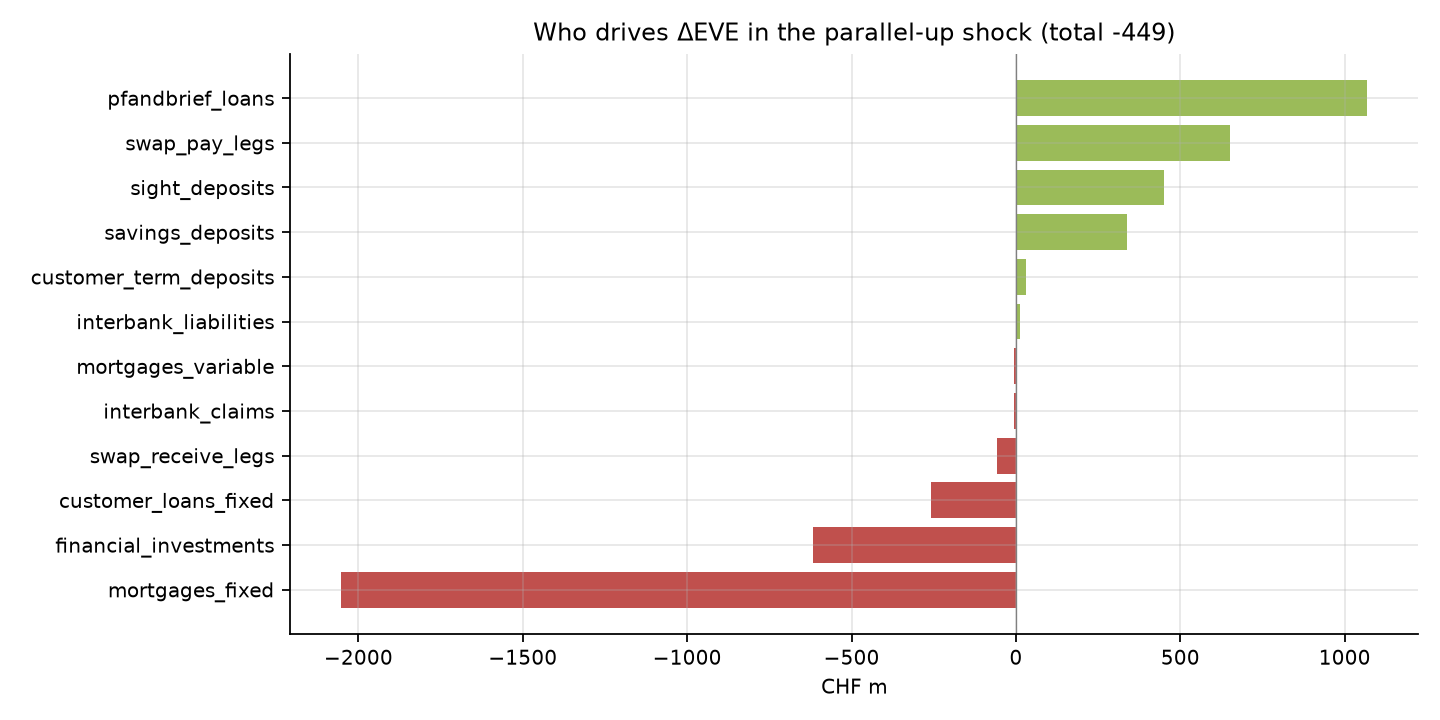
\includegraphics[width=0.85\textwidth]{fig5_eve_by_position.png}
\caption{Contribution of each balance-sheet line to \dEVE{} in the parallel-up shock.}
\label{fig:position}
\end{figure}

\subsection{Explaining the gaps}

The non-parallel shocks are less well matched: the model sees more short-rate risk ($-187$ versus $-120$ for short up) and less steepener risk ($-41$ versus $-138$). Table~\ref{tab:variants} tests four explanations. The curve matters little. Placing the volatile part of deposits at one month, as BCV does, helps slightly. Removing commercial margins from the cash flows (allowed by Basel) shrinks every number by about 20\% and fits worse, so BCV likely includes them. The largest improvement comes from the deposit split: letting the stable shares of sight and savings free, the six published figures are best matched (RMSE 29 instead of 68) with 100\% of sight deposits stable and only 16\% of savings, i.e.\ average repricing dates of 2.5 and 0.8 years instead of the published 1.8 and 1.8. Since the published averages are fixed, the gap more likely lies in the shape of BCV's replication (a moving-average volatile part and rate-dependent volumes) than in the shares themselves; the exercise shows that the twist scenarios are where the deposit model is identified.

\begin{table}[h]
\centering
\caption{\dEVE{} under alternative assumptions (CHF million) and root mean squared error against the six published figures.}
\label{tab:variants}
\small
\begin{tabular}{lrrrrrrr}
\toprule
Variant & Par.\ up & Par.\ down & Steep. & Flat. & Short up & Short down & RMSE \\
\midrule
Base model & $-449$ & 454 & $-41$ & $-49$ & $-187$ & 191 & 68 \\
Volatile deposits at 1 month & $-433$ & 438 & $-51$ & $-36$ & $-171$ & 175 & 61 \\
No commercial margin & $-361$ & 361 & $-34$ & $-39$ & $-149$ & 152 & 88 \\
Curve $+20$ bp & $-448$ & 454 & $-42$ & $-47$ & $-185$ & 189 & 67 \\
Fitted deposit shares (100\% / 16\%) & $-462$ & 478 & $-95$ & 2 & $-151$ & 154 & 29 \\
\midrule
BCV published & $-467$ & 488 & $-138$ & 40 & $-120$ & 125 & -- \\
\bottomrule
\end{tabular}
\end{table}

\subsection{Outlier test}

On BCV's own figures, the worst \dEVE{} was 13.8\%, 14.5\%, 15.02\% and 13.4\% of Tier~1 at the four reporting dates from June 2024 to December 2025 (Figure~\ref{fig:outlier}): the bank sat on the threshold in mid-2025. The ratio fell at end-2025 because the parallel-up loss shrank from 527 to 467 million. The model gives 12.9\%. With the larger shocks of the 2028 draft (175 bp parallel, 250 bp short), the model's worst \dEVE{} rises to 523 million, 15.0\% of Tier~1; simply scaling BCV's parallel-up figure by 175/150 gives 15.6\%. Unless the balance sheet or the hedges change, BCV would be at or above the outlier line under the new calibration.

\begin{figure}[t]
\centering
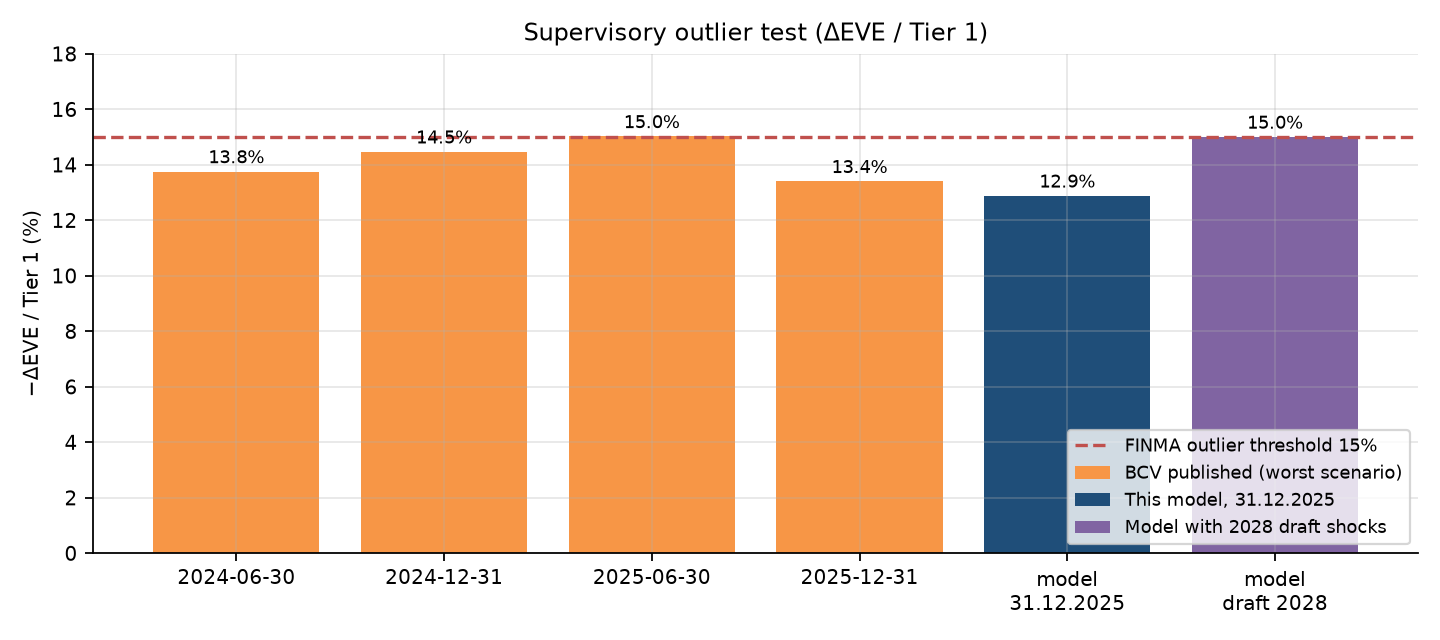
\includegraphics[width=0.85\textwidth]{fig6_outlier_test.png}
\caption{Worst \dEVE{} as a share of Tier~1: published history, model, and model under the 2028 draft shocks.}
\label{fig:outlier}
\end{figure}

\subsection{Net interest income}

In the up shock the model gains 96 million against 78 published: SNB sight deposits and swap receive legs reprice at once while deposit rates follow only partly. In the down shock the model loses 158 million against 3 published. The gap is a choice of assumption, not of arithmetic: the shock pushes the whole curve below zero, and the model's deposit rates (0.08\% on savings, 0.00\% on payment accounts) cannot fall, while assets reprice down by 150 bp. Without the floor the loss is 96 million. BCV explains its figure by gains on placing liquidity at the SNB under the exemption threshold and by negative-rate charges on part of the deposits, as in 2015--2022. Its \dNII{} therefore rests on clients accepting negative rates again, which the model does not assume.

\section{Sensitivity to the deposit model}

Because sight and savings deposits are half of the balance sheet, their modelling is the main source of uncertainty (Figure~\ref{fig:nmd}). Halving the stable share of sight deposits raises the parallel-up loss from 449 to 674 million (19.3\% of Tier~1); halving that of savings raises it to 618 million (17.7\%). The heat map shows the full trade-off: with less than about a quarter of deposits treated as stable, every replication length leaves the bank above 15\%. For earnings, the pass-through $\beta$ changes the sign of \dNII: with $\beta = 0$ the up shock adds 169 million, with $\beta = 1$ it costs 288 million; the estimated 0.35 for savings sits near the break-even point.

\begin{figure}[t]
\centering
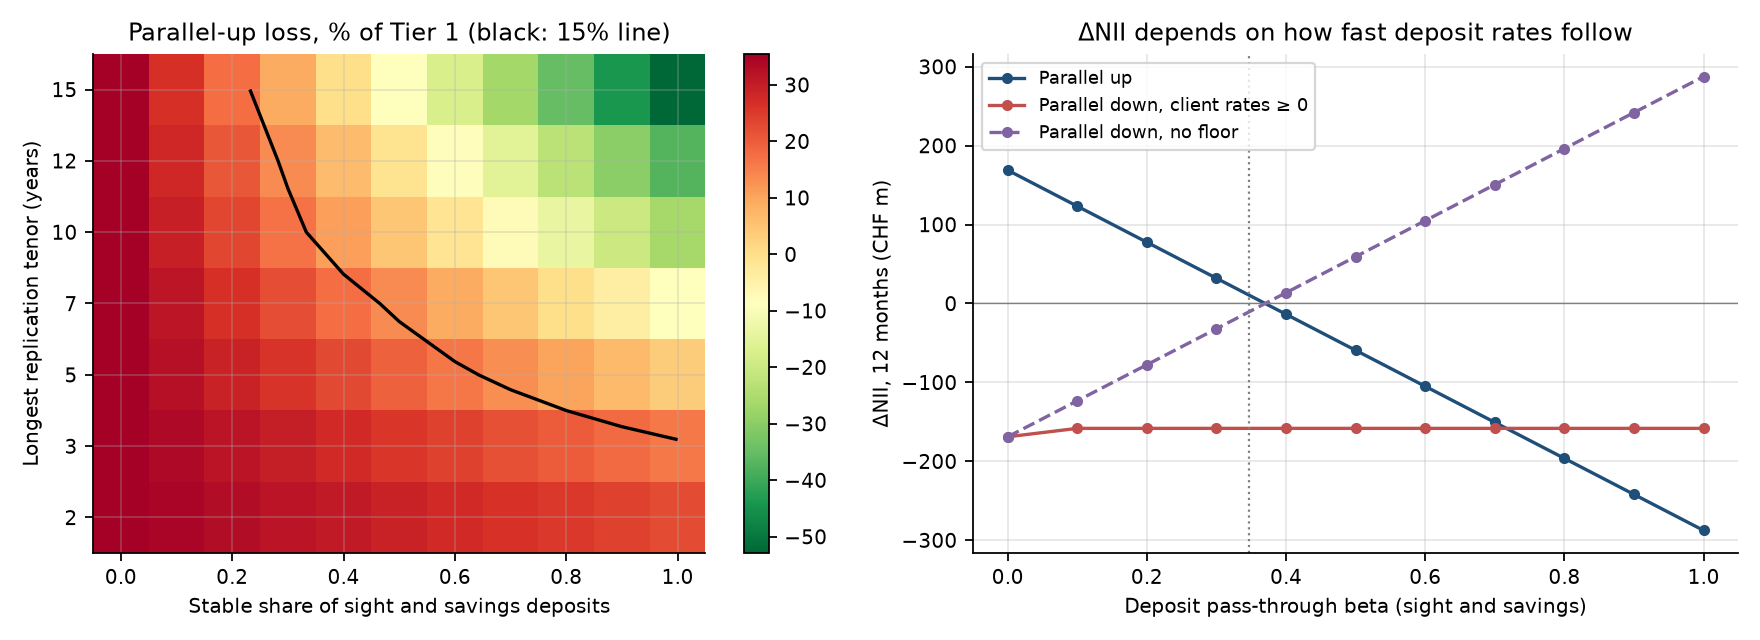
\includegraphics[width=\textwidth]{fig7_nmd_sensitivity.png}
\caption{Left: parallel-up loss as a share of Tier 1 for different stable shares and replication lengths of sight and savings deposits (same values for both). Right: \dNII{} against the deposit pass-through.}
\label{fig:nmd}
\end{figure}

\section{The mortgage prepayment option}

A borrower who repays a fixed-rate mortgage early when rates fall holds an option against the bank. BCV states that it charges a penalty equal to the lost interest margin, so prepayment leaves the bank whole and it does not model it. We test what the penalty is worth by assuming none: the fixed mortgages prepay at a constant rate (CPR) of 2\% a year plus an extra $k$ per 100 bp fall in the 5-year rate, and are repaid at par. These parameters are illustrative, not estimated. Because the stock coupon (1.81\%) is well above current market rates, the loans are worth more than par, and prepayment at par destroys that premium (Figure~\ref{fig:prepay}). With the penalty, the down shock adds 454 million to EVE. Without it, a 2\% flat CPR reduces the gain to 337 million, and a response of $k = 5\%$, 10\% or 20\% turns it into losses of 402, 997 and 1,872 million. The mortgage book shows the negative convexity familiar from US mortgages. For an auditor, the penalty clause is therefore a key assumption behind the published \dEVE{}.

\begin{figure}[t]
\centering
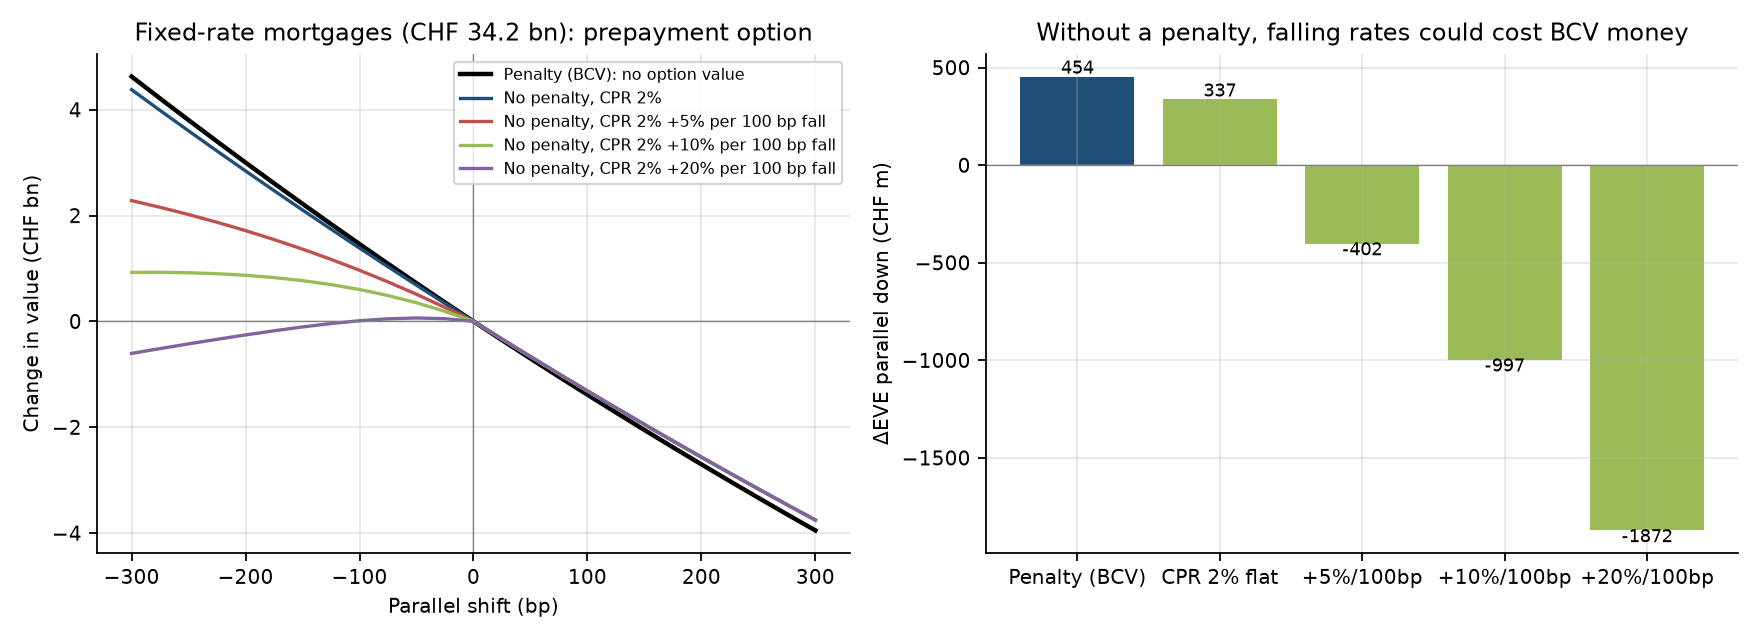
\includegraphics[width=\textwidth]{fig8_prepayment.png}
\caption{Left: value of the fixed-rate mortgage book against a parallel shift, with and without a prepayment penalty. Right: \dEVE{} of the down shock for different prepayment responses.}
\label{fig:prepay}
\end{figure}

\section{Hedging with interest rate swaps}

BCV's existing swaps are visible in IRRBBA1. Removing them from the model raises the worst \dEVE{} from 12.9\% to 29.9\% of Tier~1: the CHF 12.9 billion of payer swaps already cancel more than half of the risk. A pay-fixed, receive-SARON swap gains 72 million per billion of notional in the parallel-up shock at 5 years. To bring the worst ratio to an internal target of 10\%, the bank would need a further CHF 1.39 billion of 5-year payer swaps at the par rate of 0.10\% (Figure~\ref{fig:hedge}). The swap lowers the up-shock loss to 348 million, reduces the down-shock gain from 454 to 346, raises the up-shock \dNII{} from 96 to 117 million (the floating leg reprices at once) and worsens the down-shock \dNII{} from $-158$ to $-179$. With SARON at $-0.04\%$, the swap costs about 2 million a year of carry. Under the 2028 draft shocks the hedged ratio is 11.7\%. The trade-off is the classic one of ALM: protecting economic value against rising rates gives up part of the gain when rates fall, and makes earnings more exposed to falling rates.

\begin{figure}[t]
\centering
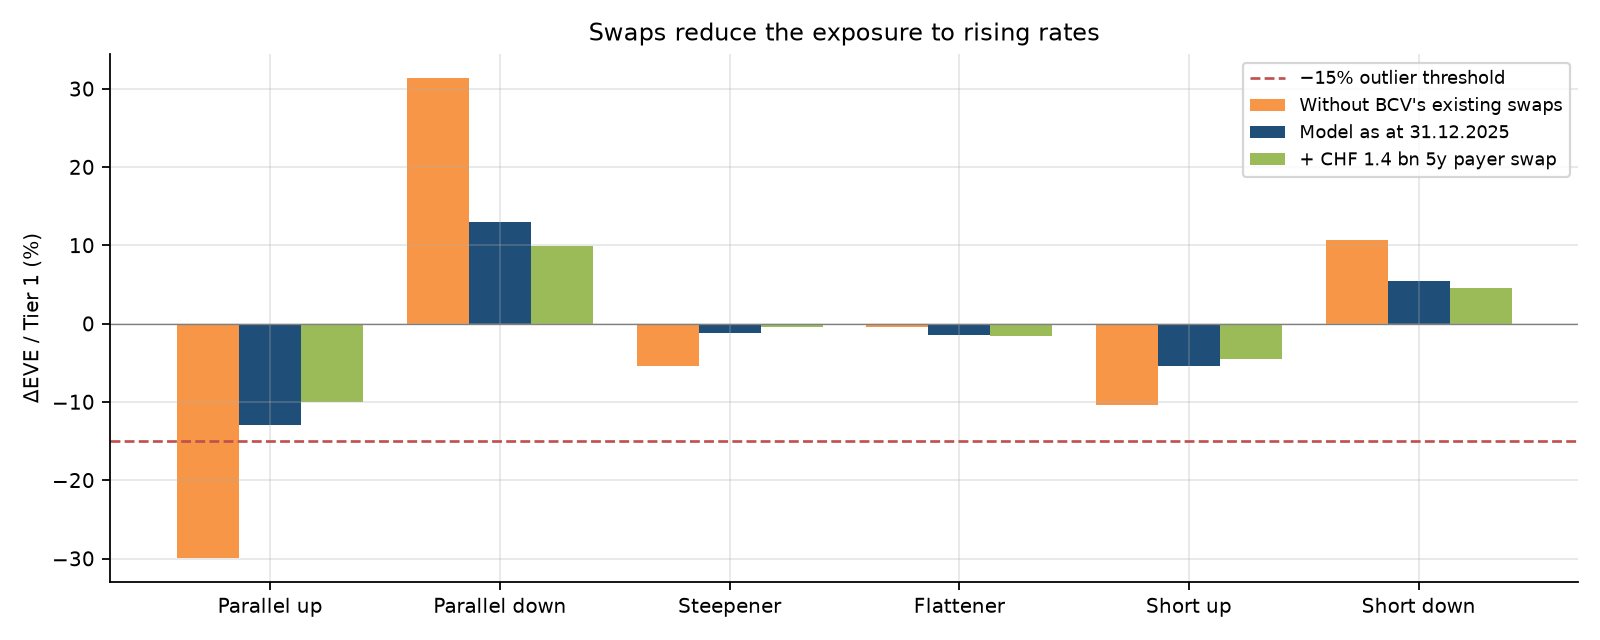
\includegraphics[width=\textwidth]{fig9_hedge.png}
\caption{\dEVE{} as a share of Tier 1 without BCV's swaps, in the base model, and with an additional 5-year payer swap.}
\label{fig:hedge}
\end{figure}

\section{Limitations}

\begin{itemize}
  \item \textbf{Aggregated data.} The model starts from 18 lines with one average repricing date each. The uniform shape of each ladder is an assumption; the true distribution of mortgage maturities is not public.
  \item \textbf{Coupons.} Stock coupons are SNB averages, not BCV's own rates. The implied run-rate net interest income (656 million) is above the reported 2025 gross interest result (519 million), so the cash flows probably carry too much margin; with no margin at all, the parallel-up \dEVE{} would be $-361$.
  \item \textbf{Curve.} Confederation bonds instead of SARON swaps, yields treated as zero rates.
  \item \textbf{Deposits.} BCV's replication model is only matched on its published averages; volumes do not react to rates.
  \item \textbf{Earnings.} Constant balance sheet, instantaneous shock, no SNB tiering, no negative-rate charges; EUR and USD positions (6\% of the balance sheet) are treated as CHF.
  \item \textbf{2028 draft.} Only the parallel and short CHF shock sizes are taken from the draft; the long shock is kept at 100 bp. The prepayment parameters are illustrative.
\end{itemize}

\section{Conclusion}

A public Pillar~3 report contains enough information to rebuild the main interest rate risk figure of a Swiss bank: from 18 lines and a free SNB curve, the model reproduces BCV's parallel-shock \dEVE{} within a few percent and confirms that the bank sits close to, but below, the 15\% outlier threshold. The exercise also shows where the number is fragile. It depends above all on how stable deposits are assumed to be; the twist scenarios reveal that BCV's deposit replication differs in shape from a simple ladder; earnings in a falling-rate scenario depend on whether clients can be charged negative rates; and the prepayment penalty protects the bank from a large option loss. Under FINMA's 2028 calibration the bank would sit at the threshold, which gives its swap programme a direct regulatory purpose. Natural extensions are loan-level maturity data, a SARON swap curve, a dynamic balance sheet for \dNII, and a behavioural deposit model with rate-dependent volumes.

\section*{Reproducibility}
All code, data and results are in the project repository. \texttt{python run\_all.py} recomputes every number and figure from the saved data and runs the 13 tests; \texttt{python run\_all.py --download} downloads the BCV, FINMA and SNB files again.

\bibliographystyle{plainnat}
\bibliography{references}

\end{document}
